\subsection{Logging Configuration}
\textit{Do the following:
\begin{itemize}
\item configure the logging using an accepted department log statement format (see Application Logging)
\item log at different logging levels (error, warn, info, debug), to see the effect of the default logging level setting
\item turn on DEBUG in the logging config to show DEBUG output
\item configure logging to go to both the console and a log file)
\end{itemize}
}

There are other logging frameworks that are easier to use and are more flexible. In addition to Java Logging API, there is also log4j, backlog, and others. They all have their own interface. When we use them, we need to import the correct classes. Changing logging libraries requires a lot of coding. Fortunately there is an over-arching library, SLF4J. It is an abstract logging API. It provides a common interface and utilizes runtime binding to use a specific logging library. Our code remains the same and we could switch out the actuall implementation library\cite{slf4j}.

\begin{figure}[H]\centering
\begin{framed}
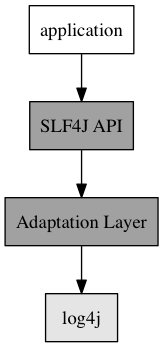
\includegraphics{slf4j.png}
\end{framed}
\caption{SLF4j Using log4j}
\label{fig:slf4jlog4j}
\end{figure}

In figure \ref{fig:slf4jlog4j} the application uses SLF4J to log. It has been bound to use log4j libraries through the adaptation layer. 

We can use the Java Logging API with SLF4J. A bit later we will swap the Java Logging API to log4j, and the code doesn't change at all.

First we will change our logging code to import the SLF4J Logger classes:
\begin{lstlisting}[language=Java]
import org.slf4j.Logger;
import org.slf4j.LoggerFactory;
\end{lstlisting}

Then we create a logger and use it to write our log messages:
\begin{lstlisting}[language=Java]
Logger logger = LoggerFactory.getLogger(this.getClass());
logger.error("Logging ERROR");
logger.warn("Logging WARN");
logger.info("Logging INFO");
logger.debug("Logging DEBUG");
\end{lstlisting}

In order to facilitate later swapping of the logging library, we will configure the logger in a configuration file. For Java Logging, the file is usually called logging.properties:
\begin{lstlisting}
handlers= java.util.logging.FileHandler, java.util.logging.ConsoleHandler
.level= FINEST

java.util.logging.FileHandler.pattern = simple.log
java.util.logging.FileHandler.limit = 50000
java.util.logging.FileHandler.count = 1
java.util.logging.FileHandler.formatter = java.util.logging.SimpleFormatter
java.util.logging.SimpleFormatter.format=%1$tb %1$td, %1$tY %1$tl:%1$tM:%1$tS %1$Tp %2$s %4$s: %5$s%n

java.util.logging.ConsoleHandler.level = FINEST
java.util.logging.ConsoleHandler.formatter = java.util.logging.SimpleFormatter
\end{lstlisting}

The first line specifies that we will use two handlers, one to log to a file and another to log to the console. The second block configures the file handler. It specifies the name of the file, formatter and the format. The last block configures the console handler to use the SimpleFormatter also.

When we want to use the logging.properties (and Java logging) with SLF4J, we need to trigger the binding by adding a VM property to tell it where the file is:
\begin{lstlisting}
java -cp ".:slf4j-jdk14-1.7.22.jar:slf4j-api-1.7.22.jar" -Djava.util.logging.config.file=./logging.properties org.familysearch.viitanenm.SimpleFormatterExample
\end{lstlisting}

We include the slf4j API library to the classpath (for our code) and also the binding library for Java Logging. Then we use the -Djava.util.logging.config.file Java Logging property to point to the configuration file.

The contents of the simple.log file with this configuration is:
\begin{lstlisting}
Dec 21, 2016 12:28:34 PM viitanenm.SimpleFormatterExample doIt SEVERE: Logging ERROR
Dec 21, 2016 12:28:35 PM viitanenm.SimpleFormatterExample doIt WARNING: Logging WARN
Dec 21, 2016 12:28:35 PM viitanenm.SimpleFormatterExample doIt INFO: Logging INFO
Dec 21, 2016 12:28:35 PM viitanenm.SimpleFormatterExample doIt FINE: Logging DEBUG
\end{lstlisting}

See how DEBUG translates into FINE level.

Java Logging has another formatter that we could use, XMLFormatter. We can swap to use it by changing the logging.properties file:

\begin{lstlisting}
java.util.logging.ConsoleHandler.formatter = java.util.logging.XMLFormatter
\end{lstlisting}

Now the output of the console handler changes to XML:
\begin{lstlisting}[language=XML]
<?xml version="1.0" encoding="UTF-8" standalone="no"?>
<!DOCTYPE log SYSTEM "logger.dtd">
<log>
<record>
  <date>2016-12-21T12:30:57</date>
  <millis>1482348657028</millis>
  <sequence>0</sequence>
  <logger>viitanenm.SimpleFormatterExample</logger>
  <level>SEVERE</level>
  <class>viitanenm.SimpleFormatterExample</class>
  <method>doIt</method>
  <thread>1</thread>
  <message>Logging ERROR</message>
</record>
<record>
  <date>2016-12-21T12:30:57</date>
  <millis>1482348657059</millis>
  <sequence>1</sequence>
  <logger>viitanenm.SimpleFormatterExample</logger>
  <level>WARNING</level>
  <class>viitanenm.SimpleFormatterExample</class>
  <method>doIt</method>
  <thread>1</thread>
  <message>Logging WARN</message>
</record>
<record>
  <date>2016-12-21T12:30:57</date>
  <millis>1482348657060</millis>
  <sequence>2</sequence>
  <logger>viitanenm.SimpleFormatterExample</logger>
  <level>INFO</level>
  <class>viitanenm.SimpleFormatterExample</class>
  <method>doIt</method>
  <thread>1</thread>
  <message>Logging INFO</message>
</record>
<record>
  <date>2016-12-21T12:30:57</date>
  <millis>1482348657060</millis>
  <sequence>3</sequence>
  <logger>viitanenm.SimpleFormatterExample</logger>
  <level>FINE</level>
  <class>viitanenm.SimpleFormatterExample</class>
  <method>doIt</method>
  <thread>1</thread>
  <message>Logging DEBUG</message>
</record>
\end{lstlisting}

There were no code changes made.

log4j is another logging library that provides more functionality than Java Logging. The code itself doesn't change at all. We just configure bindings for slf4j. If we want to use log4j logging library, for example, instead of Java Logging, we just add those libraries in our classpath.

Next we create a log4j configuration file, log4j2.properties. 

\begin{lstlisting}
# log to the console
appender.console.type = Console
appender.console.name = STDOUT
appender.console.layout.type = PatternLayout
appender.console.layout.pattern = [%d{MM-dd-yy HH:mm:ss ZZZ}] [%p] [${hostName}] %m%n

# log to a file
appender.rolling.type = RollingFile
appender.rolling.name = RollingFile
appender.rolling.fileName = mylog.log
appender.rolling.filePattern = mylog-%d{yyyy-MM-dd-HH-mm-ss}-%i.log.gz
appender.rolling.layout.type = PatternLayout
appender.rolling.layout.pattern = [%d{MM-dd-yy HH:mm:ss ZZZ}] [%p] [${hostName}] %m%n
appender.rolling.policies.type = Policies
appender.rolling.policies.time.type = TimeBasedTriggeringPolicy
appender.rolling.policies.time.interval = 2
appender.rolling.policies.time.modulate = true
appender.rolling.policies.size.type = SizeBasedTriggeringPolicy
appender.rolling.policies.size.size=500B
appender.rolling.strategy.type = DefaultRolloverStrategy
appender.rolling.strategy.max = 5
 
logger.rolling.name = com.example.my.app
logger.rolling.level = debug
logger.rolling.additivity = true
logger.rolling.appenderRef.rolling.ref = RollingFile

#set the appender
rootLogger.level = info
rootLogger.appenderRef.stdout.ref = STDOUT
rootLogger.appenderRef.rolling.ref = RollingFile
\end{lstlisting}

Slf4j follows the StringFormatter syntax, but also adds some properties. In our pattern we first print the date, time, and timezone in brackets. Then we print the log level, also in brackets. Log4j provices access to the host name or IP address with the hostName property. We print that, and in the end our customized message from the code, followed by a new line.

Log4j automatically looks for a configuration file in the path, so we don't have to specify its location when we run the code.
\begin{lstlisting}
java -cp ".:slf4j-api-1.7.22.jar:log4j-api-2.7.jar:log4j-core-2.7.jar:log4j-slf4j-impl-2.7.jar"  org.familysearch.viitanenm.ConfigLoggingExample
\end{lstlisting}

We added the log4j libraries to the classpath. We have the slf4j api library, and three libraries from log4j; log4j api library, a core library, and a binding library (to bind slf4j and log4j). 

The output will be (with info level):
\begin{lstlisting}
[12-20-16 14:41:50 -07:00] [ERROR] [viitanenm.local] Logging ERROR
[12-20-16 14:41:50 -07:00] [WARN] [viitanenm.local] Logging WARN
[12-20-16 14:41:50 -07:00] [INFO] [viitanenm.local] Logging INFO
\end{lstlisting}

In the configuration file we defined a RollingFile appender. It automatically archives the log files when they get to a specified size, or after specified time. In our example we configured it to roll when the file size is more than 500B. In pratice that limit would be larger but we just want to test it.

After running the code several times, we can see the log file rolling:
\begin{lstlisting}
-rw-r--r--   87B Dec 20 14:41 mylog-2016-12-20-14-41-29-1.log.gz
-rw-r--r--   87B Dec 20 14:41 mylog-2016-12-20-14-41-33-1.log.gz
-rw-r--r--   87B Dec 20 14:41 mylog-2016-12-20-14-41-49-1.log.gz
-rw-r--r--  143B Dec 20 14:41 mylog.log
\end{lstlisting}
